% Created 2019-02-24 Sun 22:54
% Intended LaTeX compiler: pdflatex
\documentclass[11pt]{article}
\usepackage[utf8]{inputenc}
\usepackage[T1]{fontenc}
\usepackage{graphicx}
\usepackage{grffile}
\usepackage{longtable}
\usepackage{wrapfig}
\usepackage{rotating}
\usepackage[normalem]{ulem}
\usepackage{amsmath}
\usepackage{textcomp}
\usepackage{amssymb}
\usepackage{capt-of}
\usepackage{hyperref}
\linespread{1.0}
\usepackage[left=1.5cm,right=1.5cm,top=1.5cm,bottom=1.5cm]{geometry}
\setlength{\parindent}{0in}
\setlength{\parskip}{0.15cm}
\author{eo shiru}
\date{\today}
\title{}
\hypersetup{
 pdfauthor={eo shiru},
 pdftitle={},
 pdfkeywords={},
 pdfsubject={},
 pdfcreator={Emacs 26.1 (Org mode 9.1.14)}, 
 pdflang={English}}
\begin{document}

\tableofcontents


\section{Definitionen \& Fakten}
\label{sec:org2121cbb}
\begin{itemize}
\item „A \textbf{distributed system} is a collection of independent computers that appears to its users as a single coherent system.“
\item „Ein \textbf{Verteiltes System} setzt sich aus mehreren Einzelkomponenten auf unterschiedlichen Rechnern zusammen, die in der Regel nicht über gemeinsamen Speicher verfügen und somit mittels Nachrichtenaustausch kommunizieren, um in Kooperation eine gemeinsame Zielsetzung – etwa die Realisierung einesGeschäftsablaufs – zu erreichen.“
\item A \textbf{distributed system} is a loosely coupled set of components, which run on different computers’ host systems and coordinate by means of message exchange over a communication medium to reach a common goal.
\item A \textbf{Host system} is an autonomous runtime environment, which provides a component with the necessary execution and communication resources operated by that host system.
\item Challenges when implementing a distributed system: Heterogenity, Openness, Security, Scalability, Availability/Error Handling, Concurrency, Transparency
\begin{itemize}
\item these challenges can be solved via system models (fundamental models, architectural models)
\end{itemize}
\item \textbf{Architecture} is the fundamental organization of a system embodied in its components, their relationships to each other, and to the environment, and the principles guiding its design and evolution.
\begin{itemize}
\item system = a collection of components organized to accomplish a specific function or set of functions. The term system encompasses individual applications, systems in the traditional sense, subsystems, systems of systems, product lines, product families, whole enterprises, and other aggregations of interest. A system exists to fulfill one or more missions in its environment
\item environment = determines the setting and circumstances of developmental, operational, political, and other influences upon that system
\item mission = is a use or operation for which a system is intended by one or more stakeholders to meet some set of objectives
\item stakeholder = is an individual, team, or organization (or classes thereof) with interests in, or concerns relative to, a system
\end{itemize}
\item \textbf{Architectural Styles}:
\begin{itemize}
\item N-tier Architecture
\begin{itemize}
\item Structuring of Distributed Systems into layers/levels, their distribution and interfaces
\item \textbf{Client/Server-Model}
\begin{itemize}
\item Client/Server is an example of 2-tier Architecture
\item object oriented model (units of communication \& distribution are objects)
\item component-based model (focus on reuse without the OO problems)
\end{itemize}
\item \textbf{Cluster}
\begin{itemize}
\item Set of computers/servers, which are connected to each other over a fast network and can be seen as a single unit from the outside
\end{itemize}
\end{itemize}
\item \textbf{Service-Oriented Architecture} (\textbf{SOA})  
\begin{itemize}
\item Process-oriented view with services as a base concept
\item Cross-platform/-enterprise service delivery
\item Interface reuse and interoperability
\item Composition of services (Orchestration \& Choreography)
\end{itemize}
\item Grid Computing
\begin{itemize}
\item Approach to aggregation and shared use of heterogeneous networked resources, such as computers, databases, scientific tools
\end{itemize}
\item Peer-to-Peer Architecture
\begin{itemize}
\item peers communicate with each other and offer services to their partners (peers) or use the partners’ services
\item unlike typical C/S architectures with a few servers and many clients, P2P architectures have no fixed assignment
\item Communication in P2P
\begin{itemize}
\item Service provisioning and utilization requires peer coordination
\end{itemize}
\end{itemize}
\end{itemize}
\item \textbf{Communication} is the mechanism of data exchange between components that are executed on host systems
\begin{itemize}
\item \textbf{Message Exchange Models}: Direct-Addressing-Model, Queue-Communication-Model, Port-oriented-Communication-Model, Request/Response-Model, Pull/Push-Model
\end{itemize}
\item \textbf{Middleware} = "glue"  between software components and the network ('/' slash between Client/Server); software platform bridging the heterogeneity of different systems and networks, which simultaneously provide a number of important system services, such as security policies, transaction mechanisms and directory services
\begin{itemize}
\item typical tasks/forms of middleware: RPC, MOM, EAI, Database Middleware
\begin{itemize}
\item RPC (\textbf{Remote Procedure Call})
\begin{itemize}
\item idea: "embedding" a programming language, data exchange stays transparent, RPC is located above UDP or TCP in the protocol stack, client sends RPC-request to server -> server processes and sends RPC-reply
\item enables a synchronous call of functionality offered in separate processes (possibly, on remote machines), where input and output data is exchanged over a narrow channel
\item works well with small messages and is functional foundation for lots of other middleware approaches
\item problems: requires constant encoding/decoding (marshalling), debugging is complex
\end{itemize}
\end{itemize}
\end{itemize}
\item Markup = Text that is added to the data of a document in order to convey information about it
\item Descriptive Markup = Markup that describes the structure and other attributes of a document in a non-system-specific way, independently of any processing that may be performed on it
\item Processing Instruction = Markup consisting of system-specific data that controls how a document is to be processed
\item \textbf{Design Pattern} = "describes a particular recurring design problem that arises in specific design contexts, and presents a wellproven generic scheme for its solution."
\end{itemize}
\section{URI}
\label{sec:org4a22e22}
\begin{itemize}
\item idea/goal: it must be possible to identify any resources on the internet
\item URI is generic term for all textual names/addresses
\item URI is URL or URN or URC
\item URI = Uniform Resource Identifier is a string of characters that unambiguously identifies a particular resource. To guarantee uniformity, all URIs follow a predefined set of syntax rules,[1] but also maintain extensibility through a separately defined hierarchical naming scheme (e.g. "\url{http://}")
\begin{itemize}
\item most common form of URI is the Uniform Resource Locator (URL), frequently referred to informally as a web address
\item generally 5 components: URI = scheme:[//authority]path[?query][\#fragment]
\end{itemize}
\begin{center}
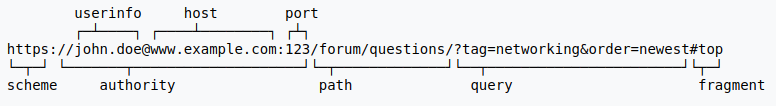
\includegraphics[width=.9\linewidth]{./uri-example.png}
\label{org94a6712}
\end{center}
\item Uniform Resource Locator (URL)
\begin{itemize}
\item The set of URI schemes that have explicit instructions on how to access the resource over the Internet
\end{itemize}
\item Uniform Resource Name (URN)
\begin{itemize}
\item A URI that has an institutional commitment to availability, etc.
\item A particular scheme intended to identify resources
\end{itemize}
\item Uniform Resource Characteristic (URC)
\begin{itemize}
\item A URC provides Meta Information
\end{itemize}
\item reserved characters in URIs: "\%" = escape character, "/" = delimiting substrings whose relationship is hierarchical, "\#" = hash fragment identifies a fragment in a resource, "?" = query delimiter to delimit the boundary between the URI of a queryable object
\item URI Syntax: <URI> ::= <scheme>":"<scheme-specific-part>
\end{itemize}

\section{HTTP}
\label{sec:org0a05f8a}
Hypertext Transfer Protocol (HTTP) is used to exchange resources (such as websites, pictures, JavaScript, other MIMEtypes resources) between a user agent and a server following the Request/Response model.
\begin{itemize}
\item developed by W3C
\item is a \emph{transfer} (not transport) protocol
\item protocol properties:
\begin{itemize}
\item exchange of Request/Response data based on TCP/IP
\item stateless communication between user agent and server
\item two message types: Request and Response
\item messages are ASCII-encoded
\item messages are used to realize methods: GET, POST, HEAD, etc
\end{itemize}
\end{itemize}

Generic Structure:
\begin{verbatim}
Start Line
*Header
CRLF
[Message-Body]
\end{verbatim}
Startline ::= Request-Line | Response-Line\\
Header ::= field-name":"[field-value]CRLF
\begin{itemize}
\item field-name = token
\item field-value = *(field-content|LWS)
\item LWS = Linear White Space
\end{itemize}
Message-Body
\begin{itemize}
\item must be encoded if exists
\item presence signaled by header field with field-name "Content-Length" or "Transfer-Encoding"
\end{itemize}

HTTP-Request Message:
\begin{verbatim}
<Method> <URI> <Protocol>
<Headers>
CRLF
[<Data>]
\end{verbatim}
Method ::= GET|POST|HEAD|\ldots{}\\
Protocol ::= HTTP/1.0 | HTTP1.1 |\ldots{}\\
Headers ::= <hName>:<hValue>\\
Data ::= <TEXT>

Example(GET):
\begin{verbatim}
GET /hello.html?parameter=value HTTP/1.1
User-Agent: Mozilla/4.0 (compatible; MSIE5.01; Windows NT)
Host: www.wikipedia.com
Accept-Language: en-us
Accept-Encoding: gzip, deflate
Connection: Keep-Alive

\end{verbatim}
Example(POST):
\begin{verbatim}
POST /guestbook.php HTTP/1.1
From: frog@jmarshall.com
Content-Type: application/x-www-form-urlencoded
Content-Length: 32

parameter=value&parameter2=value2
\end{verbatim}



HTTP-Response Message:
\begin{verbatim}
<Protocol> <Status Code> <Reason-Phrase>
<Headers>
CRLF
[<Data>]
\end{verbatim}
Protocol ::= HTTP/1.0 | HTTP1.1 |\ldots{}\\
Status-Code ::= DIGIT+\\
Reason-Phrase ::= <TEXT>\\
Headers ::= <hName>:<hValue>\\
Data ::= <TEXT>

Example:
\begin{verbatim}
HTTP/1.1 200 OK
Date: Sun, 21 Apr 1996 02:20:42 GMT
Server: Microsoft-Internet-Information-Server/5.0
Connection: keep-alive
Content-Type: text/html
Last-Modified: Thu, 18 Apr 1996 17:39:05 GMT
Content-Length: 2543

<HTML> Some data... More and more data</HTML>
\end{verbatim}

\subsection{Typical HTTP Methods}
\label{sec:orgc0f51b4}
\begin{itemize}
\item GET = deliver the resource addressed by the URI
\item POST = request to the server with respect to processing of encoded message body data (processing wrt the URI provided in POST)
\item HEAD = Like GET but without the Response Body
\item OPTIONS = Request on information submission on communication options
\item PUT = Resources encoded in the Body should be saved at the Request URI
\item DELETE = Server should remove the resources connected to the Request URI
\item TRACE = Methods for development support of the so-called application layer request loop-back; all requests of user agents that the server gets should return to the user agent
\end{itemize}

\subsection{Typical HTTP HEADERS}
\label{sec:org410e5a4}
\begin{itemize}
\item Content-Type = media type used
\item Expires = date/time from which the response is considers invalid, important for caching
\item Host = specifies internet host and port number of the requested resource
\item Last-Modified = Date and time when the “variant” (object referenced by the RequestURI) was last modified, important for caching
\item Location = Is set in the HTTP Response to notify the user agent of the new location of the requested Request-URI; Very important concept in different protocols which build up on HTTP, for example, in the security area; Is used for implementation of the so-called “Redirects”
\item Referrer = Reference to the URI from which the user agent has posted the current Request URI; Useful for maintenance/service tasks
\item User-Agent = Information about the user agent, important for personalization and internationalization
\end{itemize}

Numerous further attributes exist for use for different tasks

\subsection{HTTP Status Codes}
\label{sec:org2c8dd30}
1XX = Information as intermediate response, 2XX = Successfull operations, 200 = OK, 201 = Created, 3XX = Redirects, 301 = Moved Permanently, 302 = Moved Temporarily, 4XX = Client Error, 400 = Bad Request, 401 = Unauthorized, 403 = Forbidden, 404 = Not Found, 5XX = Server Error
\section{MIME}
\label{sec:org5605ec8}
Multipurpose Internet Mail Extension
\begin{itemize}
\item Concept
\begin{itemize}
\item MIME messages can consist of many part (-> multi-part messages)
\item message parts can have different types of content (-> Content-Type)
\item each message part has its own headers to describe the content
\end{itemize}
\item Content-Type Syntax (matching of media type and subtype is case-insensitive)
\begin{itemize}
\item content ::= "Content-Type":<type>/<subtype>[";"<parameter>]
\item type ::= discrete-type | composite-type
\item discrete-type ::= "text" | "image" | "audio" | "video" | "application" | extensions-token
\item composite-type ::= "message" | "multipart" | extensions-token
\end{itemize}
\item Example
\end{itemize}
\begin{verbatim}
Content-Type: multipart/mixed; boundary="===-1203946231==_============"

===-1203946231==_============
Content-Type: text/plain; charset="us-ascii" ; format="flowed“
===-1203946231==_============
Content-Id: <p05100306b83d3caaff11@[139.82.20.12].0.0>
Content-Type: application/vnd.ms-excel; name="WWW2002-Review-Paper-Assign.xls"
; x-mac-type="584C5334"
; x-mac-creator="5843454C"
Content-Disposition: attachment; filename="WWW2002-Review-Paper-Assign.xls"
Content-Transfer-Encoding: base64
\end{verbatim}
\section{Retrieving Information}
\label{sec:org34f9dae}
Client Side:\\
\textbf{1. Prepare Request}
\begin{itemize}
\item adress the resource (URI)
\begin{itemize}
\item find URI-resolver for scheme in use (eg uri resolver for http)
\end{itemize}
\item URI Resolver: get address of resource (scheme specific), eg. Host: localhost, Resource: /\\
\end{itemize}
\textbf{2. Request Resource}
\begin{itemize}
\item send request to address (communication)
\item depends on scheme of URI and the transmission protocol is defined by scheme
\end{itemize}

Server Side:\\
\textbf{A. Handle Request}
\begin{itemize}
\item wait for request
\begin{itemize}
\item listen on server port (usually port 80)
\item accept connection
\begin{itemize}
\item iterative server: one request after another (no concurrency)
\item concurrent server: one process/thread per request
\end{itemize}
\item Server-Loop for example: wait for connection request -> accept connection -> create thread/process -> go to server-loop
\begin{itemize}
\item Thread/Process then -> prepare processing
\end{itemize}
\end{itemize}
\item prepare processing
\begin{itemize}
\item analyse HTTP request
\begin{itemize}
\item extract URI, Host-Header, Port and analyse if they're supported allowed
\item create/call URI handler or respond with Error code
\end{itemize}
\end{itemize}
\item process/compute
\begin{itemize}
\item URI handler receives request -> wired componets are executed -> compute response
\end{itemize}
\end{itemize}
\textbf{B. Send Resource}\\
\begin{itemize}
\item URI Handler
\begin{itemize}
\item creates header for HTTP response
\item adds response resource
\item return complete response to answering process
\end{itemize}
\item answering process (eg WebServer)
\begin{itemize}
\item may create additional header elements for http response
\item sends response to client
\end{itemize}
\end{itemize}

Client Side:\\
\textbf{3. Handle Response}
\begin{itemize}
\item handle protocol eg HTTP 302 Object moved, cookies
\end{itemize}
\textbf{4. Process/Render Data of Resource}
\begin{itemize}
\item for example process header, check content-type, process resource data depending on MIME-type eg render text/html, text/text, image/gif
\end{itemize}

\section{WebSockets}
\label{sec:orgf5c4e53}
How can the server send (push) messages to the client if HTTP requires a prior Client request? The solution are WebSockets which is leaving an open TCP connection between Client and Server. WebSockets provide a persistent connection between a client and server that both parties can use to start sending data at any time.

The client establishes a WebSocket connection through a process known as the WebSocket handshake. This process starts with the client sending a regular HTTP request to the server. An Upgrade header is included in this request that informs the server that the client wishes to establish a WebSocket connection.

Here is a simplified example of the initial request headers.
\begin{verbatim}
GET ws://websocket.example.com/ HTTP/1.1
Origin: http://example.com
Connection: Upgrade
Host: websocket.example.com
Upgrade: websocket
Sec-WebSocket-Key: dGhlIHNhbXBsZSBub25jZQ== # randomly generated key, processed by server
\end{verbatim}
If the server supports the WebSocket protocol, it agrees to the upgrade and communicates this through an Upgrade header in the response.
\begin{verbatim}
HTTP/1.1 101 WebSocket Protocol Handshake
Date: Wed, 16 Oct 2013 10:07:34 GMT
Connection: Upgrade
Upgrade: WebSocket
Sec-WebSocket-Accept: s3pPLMBiTxaQ9kYGzzhZRbK+xOo= # processed key recieved from Client
\end{verbatim}
Now that the handshake is complete the initial HTTP connection is replaced by a WebSocket connection that uses the same underlying TCP/IP connection. At this point either party can starting sending data.

With WebSockets you can transfer as much data as you like without incurring the overhead associated with traditional HTTP requests. Data is transferred through a WebSocket as messages, each of which consists of one or more frames containing the data you are sending (the payload). In order to ensure the message can be properly reconstructed when it reaches the client each frame is prefixed with 4-12 bytes of data about the payload. Using this frame-based messaging system helps to reduce the amount of non-payload data that is transferred, leading to significant reductions in latency.

Advantages:
\begin{itemize}
\item Server can actively use the connection
\item No HTTP overhead
\item No delay due to polling
\end{itemize}
\section{CSS Selectors}
\label{sec:orgf26c57e}
\begin{center}
\begin{tabular}{ll}
Selector & Selects\\
\hline
\texttt{a} & selects elements with the \texttt{a} tag\\
\texttt{.red} & selects all elements with the 'red' class\\
\texttt{\#nav} & selects the elements with the 'nav' id\\
\texttt{div.row} & selects elements with \texttt{div} tag and 'row' class\\
\texttt{[aria-hidden="true"]} & selects all elements with the aria-hidden attribute with a value of “true”\\
\texttt{*} & wildcard selector that selects all elements\\
\texttt{li a} & all \texttt{a} tags that are a child of \texttt{li} tags\\
\texttt{div.row *} & selects all descendants of \texttt{div} elements with 'row' class\\
\texttt{li > a} & selects \emph{direct} descendants\\
\texttt{li + a} & selects \texttt{a} elements that are immediately preceeded by a \texttt{li} element\\
\texttt{li \textasciitilde{} a} & sibling combinator that selects all \texttt{a} elements following a \texttt{li} element\\
\texttt{li, a} & select all \texttt{a} and \texttt{li} elements\\
\texttt{p:first-child} & selects every \texttt{p} element that is first child of an element\\
\texttt{p:last-child} & selects every \texttt{p} element that is last child of an element\\
\texttt{p:nth-child(n)} & selects every \texttt{p} element that is nth child of an element\\
\texttt{a:not(.name)} & select all \texttt{a} elements that dont have the "name" class\\
\end{tabular}
\end{center}

And some common pseudo-classes: \texttt{:hover}, \texttt{:focus}, \texttt{:active}, \texttt{:link}, \texttt{:visited}

There are more CSS selectors but these are the most common ones.
\section{HTML Forms}
\label{sec:orge97d25b}
General:
\begin{verbatim}
<form
  method=“GET|POST”
  action=“URI” (E.g.:mailto:..., http:…)
  name=“form-id”
  enctype=“multipart/form-data|...”
  target=“name of frame – If used”>
Form Controls and HTML
</form>
\end{verbatim}
Example:
\begin{verbatim}
<p>Name and Age Form:</p>
<form method="POST" action= "mailto:gaedke@example.com">
  <p>Name: <input type="text" name="T1" size="20"></p>
  <p>Age:
    <select size="1" name="D1">
      <option value="15-30">29 and younger</option>
      <option value="age2">30 and above</option>
    </select>
  </p>
  <input type="submit" value="Submit" name="B1">
</form>
\end{verbatim}
\section{JS Reference}
\label{sec:org383d796}
Accessing DOM Elements
\begin{verbatim}
// Returns a reference to the element by its ID.
document.getElementById('someid');
// Returns an array-like object of all child elements which have all of the given class names.
document.getElementsByClassName('someclass');
// Returns an HTMLCollection of elements with the given tag name.
document.getElementsByTagName('LI');
// Returns the first element within the document that matches the specified group of selectors.
document.querySelector('.someclass');
// Returns a list of the elements within the document (using depth-first pre-order traversal of the document's nodes)
// that match the specified group of selectors.
document.querySelectorAll('div.note, div.alert');
// Get child nodes
var stored = document.getElementById('someid');
var children = stored.childNodes;
// Get parent node
var parental = children.parentNode;
\end{verbatim}
Creating \& Adding elements to the DOM
\begin{verbatim}
// create new elments
var newHeading = document.createElement('h1');
var newParagraph = document.createElement('p');
// create text nodes for new elements
var h1Text= document.createTextNode('This is a nice header text!');
var pText= document.createTextNode('This is a nice paragraph text!');
// attach new text nodes to new elements
newHeading.appendChild(h1Text);
newParagraph.appendChild(pText);
// elements are now created and ready to be added to the DOM.
// grab element on page you want to add stuff to
var firstHeading = document.getElementById('firstHeading');
// add both new elements to the page as children to the element we stored in firstHeading.
firstHeading.appendChild(newHeading);
firstHeading.appendChild(newParagraph);
// can also insert before like so
// get parent node of firstHeading
var parent = firstHeading.parentNode;
// insert newHeading before FirstHeading
parent.insertBefore(newHeading, firstHeading);
\end{verbatim}
Modify classes
\begin{verbatim}
firstHeading.classList.remove('foo');
firstHeading.classList.add('anotherclass');
firstHeading.classList.add('foo', 'bar');
firstHeading.classList.remove('foo', 'bar');
// if visible class is set remove it, otherwise add it
firstHeading.classList.toggle('visible');
// will return true if it has class of 'foo' or false if it does not
firstHeading.classList.contains('foo');
\end{verbatim}
Events
\begin{verbatim}
var newElement = document.getElementsByTagName('h1');
newElement.onclick = function() {
  console.log('clicked');
};
var logEventType = function(e) {
    console.log('event type:', e.type);
};
newElement.addEventListener('focus', logEventType, false);
newElement.removeEventListener('focus', logEventType, false);
window.onload = function() {
  console.log('Im loaded');
};
\end{verbatim}
Modify styles/CSS
\begin{verbatim}
myElement.style.backgroundColor = "#D93600";
// or
myElement.style.["background-color"] = "#D93600";
\end{verbatim}
\subsection{JS + Python Socket Example}
\label{sec:org671e19c}
\begin{verbatim}
// Client 1
const socket =  new WebSocket("ws://localhost:8765");
const changeSpeed = function (newspeed) {
  // send speed to websocket 
  if (socket.readyState === 1) {
    socket.send(newspeed);
  }
};
window.onbeforeunload = function () {
  socket.close();
}
// Python Server
import asyncio
import websockets
sockets = []
async def handler(websocket, path):
    sockets.append(websocket)
    async for message in websocket:
        for socket in sockets:
            await socket.send(message)
start_server = websockets.serve(handler, 'localhost', 8765)
asyncio.get_event_loop().run_until_complete(start_server)
asyncio.get_event_loop().run_forever()
// Client 2
const socket =  new WebSocket("ws://localhost:8765");
socket.onmessage = function(event) {
  changeSpeed(event.data);
}
window.onbeforeunload = function () {
  socket.close();
}
changeSpeed = function (newspeed) {
  speed = newspeed * SPEED_FAC;
}
\end{verbatim}
\subsection{JS XHR Example}
\label{sec:org9615dad}
\begin{verbatim}
const baseUrl = "https://vsr.informatik.tu-chemnitz.de/edu/2015/evs/exercises/jsajax/guestbook.php";
function loadData() {
const xhr = new XMLHttpRequest();
xhr.addEventListener("load", displayData);
xhr.open("GET", baseUrl);
xhr.send();
}
function displayData() {
  res = JSON.parse(this.responseText);
  const ul = document.getElementsByTagName("ul")[0];
  res.forEach((entry) => {
    addEntry(ul, entry);
  });
}
function addEntry(ul, entry) {
  let li = document.createElement("li");
  li.id = entry.id;
  li.innerHTML = `<strong>${entry.name}:</strong> ${entry.text} `;
  let a = document.createElement("a");
  a.setAttribute("href", entry.id);
  a.textContent = "(X)";
  li.appendChild(a);
  ul.appendChild(li);
  a.addEventListener("click", function (e) {
    e.preventDefault();
    e.stopPropagation();
    deleteEntry(this.getAttribute("href"));
  });
}
function deleteEntry(id) {
  const xhr = new XMLHttpRequest();
  xhr.open("DELETE", `${baseUrl}?id=${id}`);
  xhr.send();
  xhr.onreadystatechange = function (e) {
    if (xhr.readyState == 4 && xhr.status == 200) {
      res = JSON.parse(this.responseText);
      if (res.message) {
        li = document.getElementById(id);
        li.parentNode.removeChild(li);
      }
    }
  }
}
function sendData() {
  const xhr = new XMLHttpRequest();
  const nameEl = document.getElementById("name");
  const textEl = document.getElementById("text");
  const name = nameEl.value;
  const text = textEl.value;
  const params = `name=${name}&text=${text}`;
  nameEl.value = "";
  textEl.value = "";
  xhr.open("POST", baseUrl);
  xhr.setRequestHeader("Content-type", "application/x-www-form-urlencoded");
  xhr.send(params);
  xhr.onreadystatechange = function (e) {
    if (this.readyState == 4 && this.status == 200) {
      res = JSON.parse(this.responseText);
      const ul = document.getElementsByTagName("ul")[0];
      addEntry(ul, res.entry);
    }
  }
}
\end{verbatim}
\end{document}
